\documentclass{article}
\usepackage[utf8]{inputenc}
\usepackage{natbib}
\usepackage{graphicx}
\usepackage{geometry}
\usepackage{color}
\usepackage{float}
\usepackage{hyperref}
\usepackage{enumerate}
\usepackage{fancyhdr}
\usepackage{titling}
\usepackage{amsmath}
\usepackage{amsmath,amssymb,amsthm}
\usepackage{listings}
\usepackage[table,xcdraw]{xcolor}
\usepackage{graphicx}
\renewcommand{\baselinestretch}{1.2}%Adjust Line Spacing
\newtheorem{Q}{Question}
\geometry{left=2.5cm,right=2.5cm,top=2.5cm,bottom=2.5cm}% Adjust Margins of the File
\usepackage{tikz-qtree}
\usetikzlibrary{graphs}
\tikzset{every tree node/.style={minimum width=2em,draw,circle},
	blank/.style={draw=none},
	edge from parent/.style=
	{draw,edge from parent path={(\tikzparentnode) -- (\tikzchildnode)}},
	level distance=1.2cm}
\setlength{\droptitle}{-6em}
%%% Code style
\lstset{
	%backgroundcolor=\color{red!50!green!50!blue!50},%代码块背景色为浅灰色
	rulesepcolor= \color{gray}, %代码块边框颜色
	breaklines=true,  %代码过长则换行
	numbers=left, %行号在左侧显示
	numberstyle= \small,%行号字体
	keywordstyle= \color{magenta},%关键字颜色
	commentstyle=\color{blue}, %注释颜色
	frame=shadowbox, %用方框框住代码块
	tabsize=3, %缩进大小
	showspaces = false
}
% Create horizontal rule command with an argument of height
\newcommand{\horrule}[1]{\rule{\linewidth}{#1}}
% Set the title here
\title{
    \normalfont \normalsize
    \textsc{ShanghaiTech University} \\ [25pt]
    \horrule{0.5pt} \\[0.4cm] % Thin top horizontal rule
    \huge CS101 Algorithms and Data Structures\\ % The assignment title
    \LARGE Fall 2019\\
    \LARGE Homework 6\\
    \horrule{2pt} \\[0.5cm] % Thick bottom horizontal rule
}
% wrong usage of \author, never mind
\author{}
\date{Due date: 23:59, November 3, 2019}

% set the header and footer
\pagestyle{fancy}
\lhead{CS101 Algorithms and Data Structures}
\chead{Homework 6}
\rhead{Due date: 23:59, November 3, 2019}
\cfoot{\thepage}
\renewcommand{\headrulewidth}{0.4pt}

% special settings for the first page
\fancypagestyle{firstpage}
{
	\renewcommand{\headrulewidth}{0pt}
	\fancyhf{}
	\fancyfoot[C]{\thepage}
}

% Add the support for auto numbering
% use \problem{title} or \problem[number]{title} to add a new problem
% also \subproblem is supported, just use it like \subsection
\newcounter{ProblemCounter}
\newcounter{oldvalue}
\newcommand{\problem}[2][-1]{
	\setcounter{oldvalue}{\value{secnumdepth}}
	\setcounter{secnumdepth}{0}
	\ifnum#1>0
		\setcounter{ProblemCounter}{#1}
	\else
		\stepcounter{ProblemCounter}
	\fi
	\section{Problem \arabic{ProblemCounter}: #2}
	\setcounter{secnumdepth}{\value{oldvalue}}
}
\newcommand{\subproblem}[1]{
	\setcounter{oldvalue}{\value{section}}
	\setcounter{section}{\value{ProblemCounter}}
	\subsection{#1}
	\setcounter{section}{\value{oldvalue}}
}

\begin{document}
\maketitle
\thispagestyle{firstpage}
%\newpage
\vspace{3ex}

\begin{enumerate}
\item Please write your solutions in English. 

\item Submit your solutions to gradescope.com.  

\item Set your FULL Name to your Chinese name and your STUDENT ID correctly in Account Settings. 

\item If you want to submit a handwritten version, scan it clearly. Camscanner is recommended. 

\item When submitting, match your solutions to the according problem numbers correctly. 

\item No late submission will be accepted.

\item Violations to any of above may result in zero score. 
\end{enumerate}
\newpage

\section{(6') Graph and Disjoint Set}
Each question has one or more correct answer(s). Select all the correct answer(s). For each question, you get $0$ point if you select one or more wrong answers, but you get $0.5$ point if you select a non-empty subset of the correct answers.\\
\textit{Note that you should write you answers of section 1 in the table below.}
\begin{table}[htbp]
	\begin{tabular}{|p{2cm}|p{2cm}|p{2cm}|p{2cm}|p{2cm}|p{2cm}|}
		\hline 
		Question 1 & Question 2 & Question 3 & Question 4 & Question 5 & Question 6 \\ 
		\hline 
		&  &  &  &  &\\ 
		\hline 
	\end{tabular} 
\end{table}
\begin{Q}
Undirected Graph G = (V, E) is stored in an adjacency matrix A using 0 and 1. If we want to know whether there is a path with length m between $V_i$ and $V_j$, then we only need to check whether or not M[i][j] is zero where M is ? (if M[i][j] is 0, then this means there doesn't exist such a path)  
\begin{enumerate}[(A)]
	\item A
	\item mA
	\item $A^{m-1}$
	\item $A^m$
\end{enumerate}
\end{Q}


\begin{Q}
Which of following statements is true?
\begin{enumerate}[(A)]
	\item In a directed graph, the maximal number of edges is $|V|(|V|-1)$ 
	\item In an undirected graph, a simple path has no repetitions of edges.
	\item Both the time complexity of DFS and that of BFS are $\Theta(|V|+|E|)$ 
	\item If Graph G = (V, E) is also a tree, then $|V|$ = $|E|$ $+$ 1
\end{enumerate} 
\end{Q}


\begin{Q}
Undirected Graph G = (V, E) is stored in an adjacency matrix A. What is the degree of $V_i$?
\begin{enumerate}[(A)]
	\item $\sum_{i=1}^{|V|}$A[i][j]
	\item $\sum_{j=1}^{|V|}$A[i][j]
	\item $\sum_{i=1}^{|V|}$A[j][i]
	\item $\sum_{i=1}^{|V|}$A[i][j] + $\sum_{j=1}^{|V|}$A[j][i]
\end{enumerate}
\end{Q}

\begin{Q}
At the beginning of fall semester, Keyi, an experienced TA of CS101, was assigned a task to divide students into different discussion classes. He was a master of Data Structure and thus he decided to use disjoint sets based on votes for discussion sessions. Each class corresponds to a union tree after implementation of disjoint sets with union-by-size optimization. We know that Class1 has a union tree with height 5, thus the possible number of students in Class1 is ?     
\begin{enumerate}[(A)]
	\item 25
	\item 30
	\item 35
	\item 40
\end{enumerate}
\end{Q}
\begin{Q}
Suppose we have disjoint sets shown as the following figure. 
After we do $set\_union(e,h)$ and $find(e)$   (consider all optimization), what's the depth of node $i$?\\
A. 1 \\
B. 2 \\
C. 3 \\
D. 4 \\
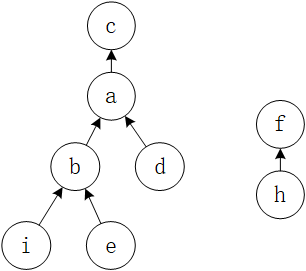
\includegraphics[scale =0.6]{fig2.png} \\
\end{Q}

\begin{Q}
Which of the following is TRUE?
\begin{enumerate}[(A)]
\item We should use an adjacency list instead of adjacency matrix to permanently store the graph in which there are 100 vertices and 200 edges 
\item Adjacency list is better than adjacency matrix when inserting a new vertex
\item We can use DFS to determine whether a graph is bipartite
\item In a connected undirected graph, we can use BFS to find the shortest path between any vertices. 
\item A directed graph with n vertices has at least n  edges to ensure the whole graph is strongly connected.
\end{enumerate}
\end{Q}
%%%%% (2)
\pagebreak
\section{(9') Weighted Graph}
A \textit{weighted graph} is a graph such that each edge has a weight (a number). The weights can be represented with an adjacency matrix, whose elements contain the weights (instead of boolean values). Note that this representation does not distinguish the case that there is an edge with weight 0 from the case that there is no edge. For this reason, we interpret a 0 in the matrix to mean that there is no edge.\\
Let A be the adjacency matrix of a weighted graph, $ G $, with the columns and rows labelled, in order, by the vertices of the set $ V = {v_0, v_1, v_2, v_3, v_4, v_5} $ That is, the first row of the matrix represents the adjacencies of vertex $v_0$, the second row those of vertex $v_1$, etc. Note that there are some non-zero diagonals which means that there are some edges of the form $(v, v)$.
$$
A = \left[
\begin{matrix}
0 & 1 & 3 & 0 & 0 & 2 \\
1 & 1 & 0 & 4 & 5 & 0 \\
3 & 0 & 0 & 5 & 4 & 0 \\
0 & 4 & 5 & 2 & 0 & 6 \\
0 & 5 & 4 & 0 & 0 & 2 \\
2 & 0 & 0 & 6 & 2 & 3
\end{matrix}
\right] 
$$
(1)(3pts) Write down the adjacency list for the graph, such that the edges in the list are ordered \textit{by increasing weight}. (If two edges have the same weight, then order them by their index order.)\\
\\
\\
\\
\\
\\
(2)(3pts) Perform a (preorder) depth first search on $G$, beginning at vertex $v_0$. Use the ordering in the adjacency list to determine the ordering of vertices visited. \\
\\
\\
\\
\\
\\
(3)(3pts) Perform a breadth first search of the graph, $ G $, again beginning at $ v_0 $ and using the ordering in the adjacency list.\\


\pagebreak

\section{(9') Disjoint Set}
Part(A): Consider a list of cities $c_1, c_2, \dots, c_n$. 
Assume we have a relation $R$ such that, for any $i,j$, $R(c_i,c_j)$ is 1
if cities $c_i$ and $c_j$ are in the same province, and 0 otherwise.\\
\\
(1)(1pts) If R is stored as a table, how much space does it require? \_\_\_\_\_\_\_\_\_\_\_\_\_\_\_\_\_\_\_\_\_\_\_\_\_\_\_\_\\
\\
(2)(2pts) Using a Disjoint Sets ADT, how do we construct it from $R$?
Briefly explain it and analyze the time complexity. (Optimization should be implemented)
\\
\\
\\
\\
\\
\\
\\
(3)(2pts) When the cities are stored in the Disjoint Sets ADT, if you are given two cities $c_i$ and $c_j$, how do you check if they are in the same province? (specific function mentioned in courseware should be used here)\\
\\
\\
\\
\\
\\
\\
Part(B): Given the following set of operations, 
show the final disjoint set tree for each of the following union strategies.\\
$set\_union(A, D),\ set\_union(C, B),\ set\_union(F, E),\ set\_union (G, C),$\\
$set\_union(D,G),\ find(A),\ set\_union(H, E),\ set\_union(E,G),\ find(E)$\\
\\
(1)(2pts) Without considering optimization. (The set specified first in the union will always be the root
of the combined set.)
\\
\\
\\
\\
\\
\\
\\
(2)(2pts) Only with path compression. (The set specified first in the union will always be
the root of the merged set.)\\




\end{document}